% !TeX program = pdflatex
\documentclass[aspectratio=169,t]{beamer}

% Idioma e Codificacao
\usepackage[brazilian]{babel}
\usepackage{booktabs}
\usepackage{array}
\usepackage{listings}
\usepackage{amsmath}
\usepackage{amssymb}
\usepackage{graphicx}
\usepackage{tikz}
\usetikzlibrary{shapes,arrows,positioning,calc,shapes.multipart}

% Carrega o Tema Modelo dos Scouts (Widescreen 16:9, Nunito Sans)
\usetheme{scouts}

% Redefine as Margens para Maximizar a Area Util de Escrita (140mm de largura util em 16:9)
\setbeamersize{text margin left=10mm, text margin right=10mm}

% Ajuste de Altura e Posicao do Titulo do Slide: Reduz Espacamento com o Topo (Cabecalho)
\setbeamerfont{frametitle}{series=\bfseries,size=\large}
\setbeamertemplate{frametitle}{%
  \vspace*{-2.5mm}% Reduz o espacamento entre o cabecalho da secao e o titulo do frame
  \begin{beamercolorbox}[wd=\textwidth,sep=0mm,left]{title}%
    \parbox[t]{\textwidth}{%
      \usebeamerfont{frametitle}\insertframetitle\strut%
    }%
  \end{beamercolorbox}%
  \vspace*{1.5mm}%
}

% Ajuste da Fonte do Comando \alert para Manter Hierarquia Visual Subordinada ao Titulo
\setbeamerfont{alerted text}{series=\bfseries,size=\footnotesize}

% Ajuste do Rodape para Liberar Mais Espaco Vertical
\setbeamertemplate{footline}{%
  \begin{beamercolorbox}[wd=\paperwidth,dp=1mm,ht=2.5mm,leftskip=10mm,rightskip=10mm]{footline}%
    \usebeamerfont{title in head/foot}\hfill%
  \end{beamercolorbox}%
}

% Ajuste Global de Fontes Beamer para Evitar Estouro de Listas Aninhadas
\setbeamerfont{itemize/enumerate body}{size=\scriptsize}
\setbeamerfont{itemize/enumerate subbody}{size=\scriptsize}
\setbeamerfont{itemize/enumerate subsubbody}{size=\tiny}
\setbeamerfont{item}{size=\scriptsize}
\setbeamerfont{subitem}{size=\tiny}

% Definicao de linguagem para MongoSH e Redis
\lstdefinelanguage{mongosh}{
  keywords={use, show, db, dbs, collections, find, findOne, insertOne, updateOne, deleteOne, aggregate, match, group, project, sort, limit, unwind, lookup, facet, explain, createIndex, ObjectId, true, false, null},
  sensitive=true,
  comment=[l]{//},
  morestring=[b]",
  morestring=[b]'
}

\lstdefinelanguage{rediscli}{
  keywords={SET, GET, MSET, MGET, INCR, DECR, EXPIRE, TTL, HSET, HGET, HGETALL, HINCRBY, LPUSH, RPUSH, LPOP, RPOP, BRPOP, SADD, SMEMBERS, SINTER, ZADD, ZRANGE, ZRANGEBYSCORE},
  sensitive=true,
  comment=[l]{\#},
  morestring=[b]",
  morestring=[b]'
}

% Configuracao Geral de Listagens
\lstset{
    basicstyle=\fontsize{5.2pt}{6.3pt}\selectfont\ttfamily,
    keywordstyle=\bfseries\color{ScoutNavy},
    stringstyle=\color{ScoutGreen},
    commentstyle=\itshape\color{gray},
    backgroundcolor=\color{black!3},
    frame=single,
    rulecolor=\color{black!15},
    breaklines=true,
    breakatwhitespace=true,
    showstringspaces=false,
    tabsize=2,
    aboveskip=2pt,
    belowskip=1pt,
    literate={á}{{\'a}}1 {ã}{{\~a}}1 {â}{{\^a}}1 {à}{{\`a}}1
             {é}{{\'e}}1 {ê}{{\^e}}1 {í}{{\'i}}1 {ó}{{\'o}}1
             {õ}{{\~o}}1 {ô}{{\^o}}1 {ú}{{\'u}}1 {ç}{{\c{c}}}1
             {Á}{{\'A}}1 {Ã}{{\~A}}1 {É}{{\'E}}1 {Í}{{\'I}}1
             {Ó}{{\'O}}1 {Õ}{{\~O}}1 {Ú}{{\'U}}1 {Ç}{{\c{C}}}1
}

% Metadados Institucionais
\author{Prof. Me. Reginaldo Fernandes}
\institute{Instituto Federal do Ceará -- Campus Tauá \\ Tecnologia em Análise e Desenvolvimento de Sistemas}
\title{Bancos de Dados Não-Relacionais}
\subtitle{Aula 09: Laboratório de Fixação e Revisão Integrada (Redis + MongoDB) -- Sábado Letivo}
\date{14 de Novembro de 2026}

\begin{document}
\shorthandoff{"}

% ------------------------------------------------------------------------------
% Capa da Apresentacao
% ------------------------------------------------------------------------------
\changecolours[inverse]{ScoutGreen}
\frame[plain]{\titlepage}

% ------------------------------------------------------------------------------
% Sumario Executivo da Aula
% ------------------------------------------------------------------------------
\changecolours{ScoutGreen}
\begin{frame}{Roteiro de Revisão e Simulado N1}
  \vspace{0.3cm}
  \tableofcontents
\end{frame}

% ------------------------------------------------------------------------------
% Modulos da Aula
% ------------------------------------------------------------------------------
% !TeX root = main.tex
\changecolours{ScoutGreen}
\section[Visão Geral da Revisão N1]{Visão Geral da Revisão Integrada N1}

% ------------------------------------------------------------------------------
\begin{frame}{Objetivos do Sábado Letivo: Revisão e Simulado}
  \vspace{0.1cm}
  \begin{columns}[t,onlytextwidth]
    \begin{column}{0.48\textwidth}
      \alert{Propósito do Encontro}\par
      \footnotesize
      \begin{itemize}
        \item Consolidar o conteúdo integral do 1º Período Letivo (Aulas 01 a 08).
        \item \textbf{Sem conteúdo novo:} foco total em resolução prática e fixação de conceitos.
        \item Preparação imediata para os exames:
          \begin{itemize}
            \item \textbf{AVP1 (Aula 10):} Avaliação prática em laboratório com Redis e MongoDB.
            \item \textbf{AVT1 (Aula 11):} Avaliação teórica individual e entrega da Lista 1.
          \end{itemize}
      \end{itemize}
    \end{column}
    \begin{column}{0.48\textwidth}
      \alert{Matriz de Competências de N1}\par
      \footnotesize
      \begin{itemize}
        \item \textbf{Teoria:} Teorema CAP, Teorema PACELC e Propriedades ACID vs BASE.
        \item \textbf{Redis:} Chave-Valor, TTL, Hashes, Filas e Padrão Cache-Aside.
        \item \textbf{MongoDB:} BSON, Atualizações Atômicas, Regra ESR e Covered Queries.
        \item \textbf{Analytics:} Aggregation Framework e Pipelines no MongoDB.
      \end{itemize}
    \end{column}
  \end{columns}
\end{frame}

% ------------------------------------------------------------------------------
\begin{frame}{Arquitetura Integrada do Simulado: Cache-Aside}
  \vspace{-0.1cm}
  \centering
  \begin{tikzpicture}[
    box/.style={rectangle, draw=ScoutNavy, rounded corners=3pt, text centered, minimum height=1.0cm, line width=0.8pt, font=\scriptsize\bfseries},
    arrow/.style={thick, ->, >=stealth, color=ScoutGreen!85!black},
    lbl/.style={font=\tiny\bfseries, color=ScoutNavy!90, fill=white, inner sep=1.5pt}
  ]
    \node [box, fill=ScoutNavy!15, text width=2.8cm] (app) at (0, 0) {Aplicação Python\\(FastAPI / PyMongo)};
    \node [box, fill=ScoutGreen!20, text width=2.6cm] (redis) at (6.0, 0) {Redis 7.4\\(Cache em RAM / TTL)};
    \node [box, fill=ScoutGreen!35, text width=2.6cm] (mongo) at (6.0, -1.8) {MongoDB 8.0\\(Disco / BSON)};
    
    % Conexões App <-> Redis
    \draw [arrow] ([yshift=3pt]app.east) -- node[above, lbl] {1. Consulta Cache} ([yshift=3pt]redis.west);
    \draw [arrow, dashed] ([yshift=-3pt]redis.west) -- node[below, lbl] {Cache Hit ($<0.1\text{ ms}$)} ([yshift=-3pt]app.east);
    
    % Conexões App -> Mongo e Mongo -> Redis
    \draw [arrow] (app.south) |- node[near end, below, lbl] {2. Cache Miss: Lê Primário} (mongo.west);
    \draw [arrow] (mongo.north) -- node[right, lbl] {3. Salva no Cache com TTL} (redis.south);
  \end{tikzpicture}

  \vspace{0.25cm}
  \begin{columns}[t,onlytextwidth]
    \begin{column}{0.48\textwidth}
      \alert{Mecanismo de Consulta e Escrita}\par
      \footnotesize
      \begin{itemize}
        \item \textbf{Cache Hit:} Resposta instantânea em submilisegundo direto da RAM.
        \item \textbf{Cache Miss:} Busca indexada no MongoDB ($B\text{-Tree}$) e hidratação do Redis.
      \end{itemize}
    \end{column}
    \begin{column}{0.48\textwidth}
      \alert{Invalidação e Consistência}\par
      \footnotesize
      \begin{itemize}
        \item \textbf{Invalidação:} Deleção atômica da chave do Redis em alterações no MongoDB.
        \item \textbf{TTL Expirável:} Garante expiração automática contra dados obsoletos.
      \end{itemize}
    \end{column}
  \end{columns}
\end{frame}

% !TeX root = main.tex
\changecolours{ScoutNavy}
\section[Fundamentos Teóricos: CAP, PACELC e ACID/BASE]{Fundamentos Teóricos: Teoremas CAP, PACELC e Modelo ACID vs BASE}

% ------------------------------------------------------------------------------
\begin{frame}{Revisão do Teorema CAP (Eric Brewer, 2000)}
  \vspace{0.1cm}
  \begin{columns}[t,onlytextwidth]
    \begin{column}{0.48\textwidth}
      \alert{Os Três Pilares Fundamentais}\par
      \footnotesize
      \begin{itemize}
        \item \textbf{C (Consistência Forte):} Todos os nós retornam o dado mais recente ou geram erro imediato.
        \item \textbf{A (Disponibilidade):} Todo nó ativo responde a qualquer requisição sem retornar erro.
        \item \textbf{P (Tolerância a Partições):} O sistema continua operando mesmo sob perda ou atraso de pacotes na rede.
      \end{itemize}
      
      \vspace{0.15cm}
      \textbf{Princípio Físico:} Partições de rede são inevitáveis ($P$), forçando o arquiteto a escolher estritamente entre \textbf{CP} ou \textbf{AP}.
    \end{column}
    
    \begin{column}{0.48\textwidth}
      \alert{Classificação Arquitetural e Trade-offs}\par
      \footnotesize
      \begin{itemize}
        \item \textbf{Sistemas CP (Consistência):} Priorizam a verdade dos dados. Sob partição, bloqueiam escritas em nós isolados para impedir divergências (\textit{split-brain}). \textbf{Ex.: MongoDB}.
        
        \item \textbf{Sistemas AP (Disponibilidade):} Priorizam disponibilidade contínua. Aceitam escritas mesmo desconectados, convergindo depois via consistência eventual. \textbf{Ex.: Cassandra, DynamoDB}.
      \end{itemize}
    \end{column}
  \end{columns}
\end{frame}

% ------------------------------------------------------------------------------
\begin{frame}{O Teorema PACELC (Daniel Abadi, 2012)}
  \vspace{0.1cm}
  \begin{columns}[t,onlytextwidth]
    \begin{column}{0.41\textwidth}
      \alert{Extensão do Teorema CAP}\par
      \footnotesize
      O CAP cobre apenas o sistema em partição. O PACELC detalha também o regime operacional normal:
      \begin{itemize}
        \item \textbf{Se Partição (\textbf{P}):} Escolhe-se entre Disponibilidade (\textbf{A}) ou Consistência (\textbf{C});
        \item \textbf{Senão (\textbf{E}lse -- normal):} Escolhe-se entre Latência (\textbf{L}) ou Consistência (\textbf{C}).
      \end{itemize}
      
      \vspace{0.1cm}
      $\implies$ \textbf{Trade-off:} Garantir consistência entre réplicas síncronas exige maior latência.
    \end{column}
    
    \begin{column}{0.56\textwidth}
      \alert{Mapeamento Prático dos Bancos}\par
      \vspace{0.4cm}
      \scriptsize
      \begin{tabular}{@{}llp{3.8cm}@{}}
        \toprule
        \textbf{Banco} & \textbf{Classif.} & \textbf{Comportamento em Produção} \\
        \midrule
        \textbf{MongoDB}   & \textbf{PC/EC} & Consistência primária e sob partição \\
        \textbf{Redis}     & \textbf{PA/EL} & Latência mínima ($\approx 0.1\text{ ms}$) e alta disp. \\
        \textbf{Cassandra} & \textbf{PA/EL} & Consistência eventual com baixa latência \\
        \bottomrule
      \end{tabular}
    \end{column}
  \end{columns}
\end{frame}

% ------------------------------------------------------------------------------
\begin{frame}{Transações ACID versus Modelo BASE}
  \vspace{0.1cm}
  \begin{columns}[t,onlytextwidth]
    \begin{column}{0.48\textwidth}
      \alert{Propriedades ACID (RDBMS / Relacional)}\par
      \footnotesize
      \begin{itemize}
        \item \textbf{Atomicidade:} Todas as operações executam com sucesso ou sofrem reversão total (\textit{rollback}).
        \item \textbf{Consistência:} Respeito estrito a restrições de integridade, tipos e chaves estrangeiras.
        \item \textbf{Isolamento:} Transações concorrentes não interferem nos resultados intermediários mútuos.
        \item \textbf{Durabilidade:} Confirmação persistida em disco permanentemente após o \textit{commit}.
      \end{itemize}
    \end{column}
    
    \begin{column}{0.48\textwidth}
      \alert{Propriedades BASE (NoSQL / Distribuído)}\par
      \footnotesize
      \begin{itemize}
        \item \textbf{Basically Available:} Disponibilidade básica assegurada mesmo com nós degradados.
        \item \textbf{Soft State:} O estado dos dados pode sofrer variações temporárias sem requisições do usuário.
        \item \textbf{Eventual Consistency:} Se nenhuma nova escrita ocorrer, todas as réplicas convergem para o mesmo valor.
      \end{itemize}
    \end{column}
  \end{columns}
\end{frame}

% !TeX root = main.tex
\changecolours{ScoutRed}
\section[Revisão Redis: Estruturas e TTL]{Revisão do Redis: Estruturas de Dados, Caching e Filas}

% ------------------------------------------------------------------------------
\begin{frame}[fragile]{As Cinco Estruturas Nativas do Redis}
  \vspace{0.1cm}
  \alert{Quadro Sinóptico de Estruturas em Memória RAM}\par
  \vspace{0.3cm}
  \scriptsize
  \begin{tabular}{@{}llp{7.8cm}@{}}
    \toprule
    \textbf{Estrutura} & \textbf{Comandos Principais} & \textbf{Cenário de Aplicação Típico} \\
    \midrule
    \textbf{Strings}     & \lstinline[language=rediscli, basicstyle=\scriptsize\ttfamily]|SET, GET, INCR, MGET|       & Cache simples, tokens JWT de sessão, contadores atômicos \\
    \textbf{Hashes}      & \lstinline[language=rediscli, basicstyle=\scriptsize\ttfamily]|HSET, HGET, HGETALL|       & Objetos e entidades (ex.: carrinho, perfil de usuário) \\
    \textbf{Lists}       & \lstinline[language=rediscli, basicstyle=\scriptsize\ttfamily]|LPUSH, RPOP, BRPOP|        & Filas assíncronas FIFO, desacoplamento produtor/consumidor \\
    \textbf{Sets}        & \lstinline[language=rediscli, basicstyle=\scriptsize\ttfamily]|SADD, SMEMBERS, SINTER|    & Tags exclusivas, relacionamentos e conjuntos matemáticos \\
    \textbf{Sorted Sets} & \lstinline[language=rediscli, basicstyle=\scriptsize\ttfamily]|ZADD, ZRANGE, ZREVRANGE|   & Rankings analíticos (\textit{leaderboards}), pontuações por score \\
    \bottomrule
  \end{tabular}
  
  \vspace{0.35cm}
  \alert{Complexidade Assintótica e Performance}\par
  \footnotesize
  O acesso por chave no Redis opera com complexidade $\mathcal{O}(1)$ em memória RAM, viabilizando latências de leitura e escrita inferiores a $0.1\text{ ms}$.
\end{frame}

% ------------------------------------------------------------------------------
\begin{frame}[fragile]{Estratégia de Expiração (TTL) e Persistência}
  \vspace{0.1cm}
  \begin{columns}[t,onlytextwidth]
    \begin{column}{0.48\textwidth}
      \alert{Mecanismos de TTL e Expiração}\par
      \footnotesize
      \begin{itemize}
        \item \lstinline[language=rediscli, basicstyle=\footnotesize\ttfamily]|EXPIRE chave seg|: define tempo de validade do dado.
        \item \lstinline[language=rediscli, basicstyle=\footnotesize\ttfamily]|TTL chave|: retorna segundos restantes ($-2$ se expirou, $-1$ se sem TTL).
        \item \textbf{Gestão de RAM:} Evita retenção indevida de chaves voláteis.
      \end{itemize}
      
      \vspace{0.15cm}
      \alert{Persistência: RDB vs AOF}\par
      \begin{itemize}
        \item \textbf{RDB (Snapshot):} Imagens compactas em intervalos configurados.
        \item \textbf{AOF (Append Only):} Registro cronológico para durabilidade estrita.
      \end{itemize}
    \end{column}
    
    \begin{column}{0.50\textwidth}
      \alert{Demonstração Prática no redis-cli}\par
      \vspace{0.05cm}
      \begin{lstlisting}[language=rediscli]
# Gravacao com expiracao atomica de 60s
SET produto:SKU-001 "Notebook" EX 60

# Consulta de tempo restante de vida
TTL produto:SKU-001

# Carrinho em Hash com incremento atomico
HSET carrinho:user_12 sku "SKU-001"
HINCRBY carrinho:user_12 quantidade 1
HGETALL carrinho:user_12

# Fila assincrona FIFO (Produtor / Consumidor)
LPUSH fila:checkout "PED-2026-001"
BRPOP fila:checkout 0
      \end{lstlisting}
    \end{column}
  \end{columns}
\end{frame}

% !TeX root = main.tex
\changecolours{ScoutTeal}
\section[Revisão MongoDB: CRUD e ESR]{Revisão do MongoDB: Modelagem, CRUD Atômico e Índices ESR}

% ------------------------------------------------------------------------------
\begin{frame}[fragile]{Decisões de Modelagem: Incorporação vs Referenciamento}
  \vspace{0.1cm}
  \begin{columns}[t,onlytextwidth]
    \begin{column}{0.48\textwidth}
      \alert{Incorporação (\textit{Embedding})}\par
      \footnotesize
      \begin{itemize}
        \item Cardinalidades \textbf{1:1} e \textbf{1:Poucos} (\textit{1:Few}).
        \item Leitura atômica de documento único sem junções em disco.
        \item Limite máximo físico de 16 MB por documento BSON.
        \item Indicado para dados consultados em conjunto (ex.: itens de pedido).
      \end{itemize}
    \end{column}
    
    \begin{column}{0.48\textwidth}
      \alert{Referenciamento (\textit{Referencing})}\par
      \footnotesize
      \begin{itemize}
        \item Cardinalidades \textbf{1:Muitos} e \textbf{1:Infinitos} (\textit{1:Squillions}).
        \item Evita replicação excessiva e anomalias de atualização.
        \item Uso do \lstinline[language=mongosh, basicstyle=\footnotesize\ttfamily]|ObjectId| de 12 bytes como chave primária.
        \item Indicado para entidades grandes e independentes (ex.: clientes e catálogo).
      \end{itemize}
    \end{column}
  \end{columns}
\end{frame}

% ------------------------------------------------------------------------------
\begin{frame}[fragile]{Operadores de Atualização Atômica e Filtros em Arrays}
  \vspace{0.1cm}
  \begin{columns}[t,onlytextwidth]
    \begin{column}{0.48\textwidth}
      \alert{Atomicidade e Operadores de Modificação}\par
      \footnotesize
      \begin{itemize}
        \item O MongoDB garante atomicidade no nível de documento único sem transações pesadas distribuídas.
        \item \lstinline[language=mongosh, basicstyle=\footnotesize\ttfamily]|$set|: altera campos específicos pontualmente.
        \item \lstinline[language=mongosh, basicstyle=\footnotesize\ttfamily]|$inc|: incremento atômico de contadores ou saldos.
        \item \lstinline[language=mongosh, basicstyle=\footnotesize\ttfamily]|$elemMatch|: evita falsos positivos em arrays de subdocumentos.
      \end{itemize}
    \end{column}
    
    \begin{column}{0.50\textwidth}
      \alert{Demonstração no MongoSH}\par
      \vspace{0.05cm}
      \begin{lstlisting}[language=mongosh]
// Filtro rigoroso com $elemMatch no array
db.pedidos.find({
  itens: {
    $elemMatch: {
      preco_unitario: { $gte: 100.0 },
      quantidade: { $gte: 2 }
    }
  }
});

// Atualizacao atomica de estoque com $inc
db.produtos.updateOne(
  { sku: "SKU-ELE-001" },
  { $inc: { estoque: -1 } }
);
      \end{lstlisting}
    \end{column}
  \end{columns}
\end{frame}

% ------------------------------------------------------------------------------
\begin{frame}[fragile]{A Regra de Ouro ESR (\textit{Equality, Sort, Range})}
  \vspace{0.1cm}
  \begin{columns}[t,onlytextwidth]
    \begin{column}{0.50\textwidth}
      \alert{Ordem Estrita dos Campos no Índice Composto}\par
      \footnotesize
      \begin{enumerate}
        \item \textbf{E (Equality):} Predicados de igualdade exata (ex.: \lstinline[language=mongosh, basicstyle=\footnotesize\ttfamily]|status: "entregue"|).
        \item \textbf{S (Sort):} Campos de ordenação (\lstinline[language=mongosh, basicstyle=\footnotesize\ttfamily]|data_pedido: -1|). Elimina ordenação em RAM (\lstinline[language=mongosh, basicstyle=\footnotesize\ttfamily]|SORT|).
        \item \textbf{R (Range):} Faixas de valores (\lstinline[language=mongosh, basicstyle=\footnotesize\ttfamily]|$gte|, \lstinline[language=mongosh, basicstyle=\footnotesize\ttfamily]|$lt|, \lstinline[language=mongosh, basicstyle=\footnotesize\ttfamily]|$in|).
      \end{enumerate}
      
      \vspace{0.15cm}
      \alert{Diagnóstico com \lstinline[language=mongosh, basicstyle=\footnotesize\ttfamily]|explain()|}\par
      \footnotesize
      \begin{itemize}
        \item Proporção ideal: $\frac{\text{totalDocsExamined}}{\text{nReturned}} \to 1$.
        \item Elimina varredura total (\lstinline[language=mongosh, basicstyle=\footnotesize\ttfamily]|COLLSCAN|).
      \end{itemize}
    \end{column}
    
    \begin{column}{0.48\textwidth}
      \alert{Pipeline ESR Otimizado}\par
      \vspace{0.05cm}
      \begin{lstlisting}[language=mongosh]
// 1. Criacao do indice composto ESR
db.pedidos.createIndex({
  status: 1,        // Equality
  data_pedido: -1,  // Sort
  valor_total: 1    // Range
});

// 2. Consulta otimizada aproveitando indice
db.pedidos.find({
  status: "entregue",
  valor_total: { $gte: 300.0 }
}).sort({ data_pedido: -1 });
      \end{lstlisting}
    \end{column}
  \end{columns}
\end{frame}

% !TeX root = main.tex
\changecolours{ScoutPurple}
\section[Aggregation e Desafio Integrado]{Aggregation Framework, Performance e Desafio Prático}

% ------------------------------------------------------------------------------
\begin{frame}[fragile]{Revisão do Aggregation Framework: Estrutura em Pipeline}
  \vspace{0.1cm}
  \begin{columns}[t,onlytextwidth]
    \begin{column}{0.48\textwidth}
      \alert{Estágios Críticos do Pipeline}\par
      \footnotesize
      \begin{itemize}
        \item \lstinline[language=mongosh, basicstyle=\footnotesize\ttfamily]|$match|: redução inicial volumétrica via índice $B\text{-Tree}$.
        \item \lstinline[language=mongosh, basicstyle=\footnotesize\ttfamily]|$unwind|: desconstrução de arrays para permitir agregações por item.
        \item \lstinline[language=mongosh, basicstyle=\footnotesize\ttfamily]|$group|: agrupamento por chave e acumuladores (\lstinline[language=mongosh, basicstyle=\footnotesize\ttfamily]|$sum|, \lstinline[language=mongosh, basicstyle=\footnotesize\ttfamily]|$avg|).
        \item \lstinline[language=mongosh, basicstyle=\footnotesize\ttfamily]|$sort| e \lstinline[language=mongosh, basicstyle=\footnotesize\ttfamily]|$limit|: ordenação determinística e paginação.
      \end{itemize}
    \end{column}
    
    \begin{column}{0.50\textwidth}
      \alert{Pipeline Analítico no MongoSH}\par
      \vspace{0.05cm}
      \begin{lstlisting}[language=mongosh]
// Relatorio de faturamento por categoria
db.pedidos.aggregate([
  { $match: { status: "ENTREGUE" } },
  { $unwind: "$itens" },
  {
    $group: {
      _id: "$itens.categoria",
      receita: { $sum: "$itens.subtotal" },
      unidades: { $sum: "$itens.quantidade" }
    }
  },
  { $sort: { receita: -1 } }
]);
      \end{lstlisting}
    \end{column}
  \end{columns}
\end{frame}

% ------------------------------------------------------------------------------
\begin{frame}{Evidência Empírica: Latência Poliglota Integrada}
  \vspace{0.1cm}
  \begin{columns}[t,onlytextwidth]
    \begin{column}{0.48\textwidth}
      \alert{Comparativo das Camadas de Acesso}\par
      \footnotesize
      \begin{itemize}
        \item \textbf{Redis (RAM):} $\approx 0.08\text{ ms}$ (acesso $\mathcal{O}(1)$ via chave direta). Mais de $200\times$ mais rápido que disco.
        \item \textbf{MongoDB Indexado ($B\text{-Tree}$):} $\approx 1.15\text{ ms}$ ($\mathcal{O}(\log N)$ via índice composto ESR).
        \item \textbf{MongoDB sem Índice (\texttt{COLLSCAN}):} $\approx 18.4\text{ ms}$ ($\mathcal{O}(N)$ varredura linear de $10.000$ docs).
      \end{itemize}
      
      \vspace{0.15cm}
      \alert{Conclusão de Arquitetura}\par
      A arquitetura de cache-aside combina a velocidade em RAM do Redis com a persistência de documentos do MongoDB.
    \end{column}
    
    \begin{column}{0.50\textwidth}
      \alert{Medição Empírica (Tempo de Resposta)}\par
      \vspace{0.05cm}
      \centering
      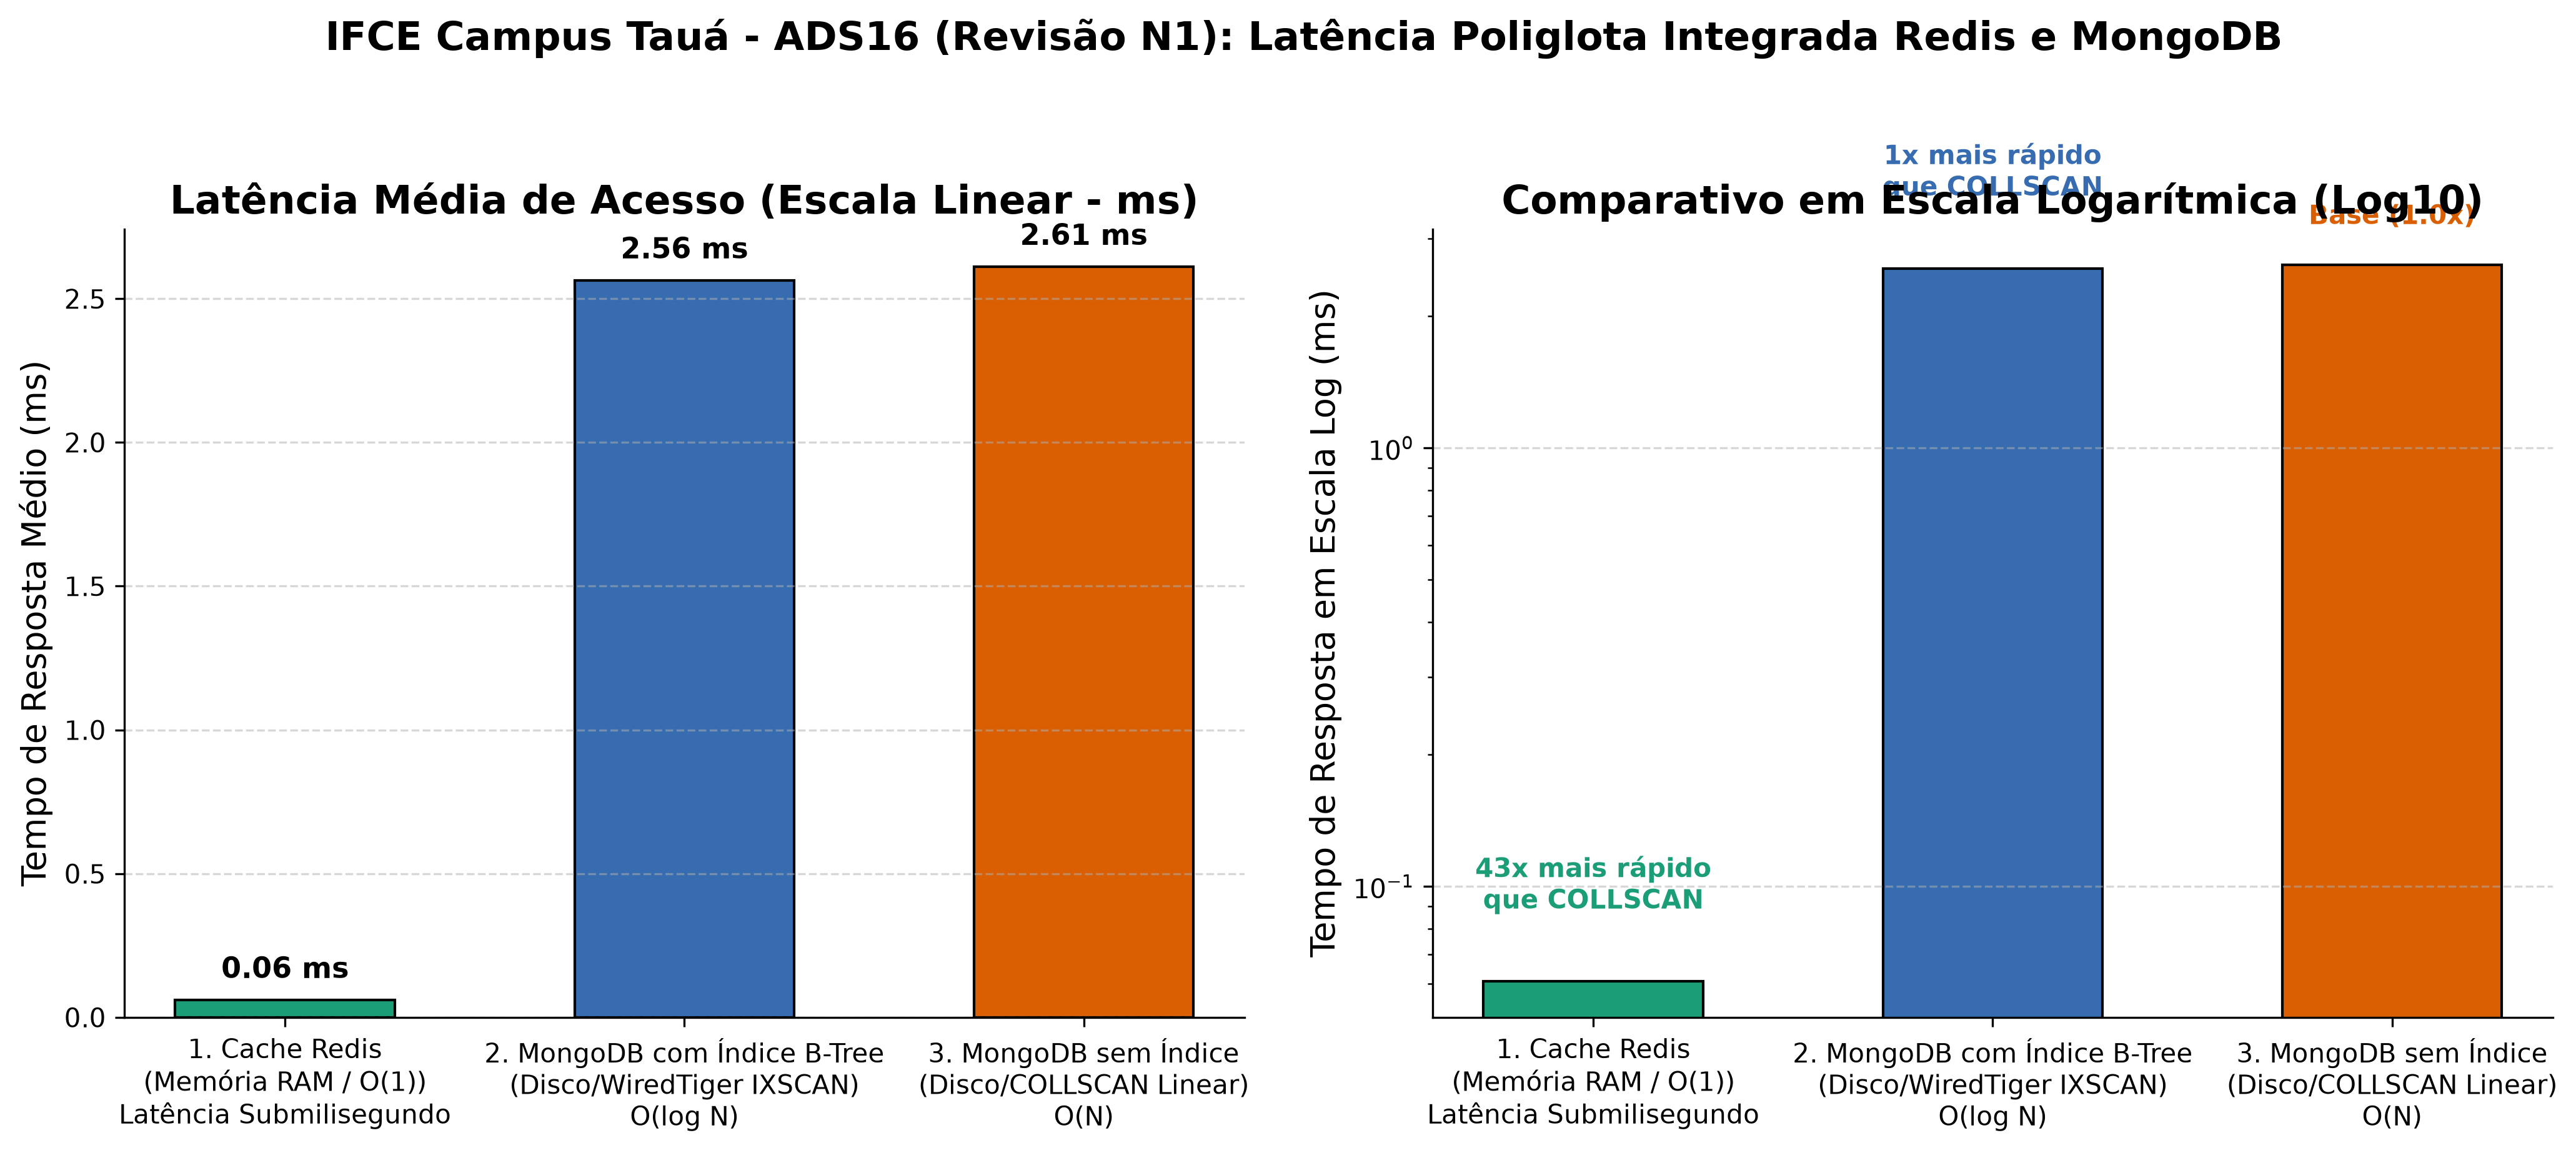
\includegraphics[width=\linewidth, height=4.2cm, keepaspectratio]{benchmark_latencia_revisao.png}
    \end{column}
  \end{columns}
\end{frame}

% ------------------------------------------------------------------------------
\begin{frame}[fragile]{Diretrizes para o Simulado Prático (AVP1)}
  \vspace{0.1cm}
  \begin{columns}[t,onlytextwidth]
    \begin{column}{0.48\textwidth}
      \alert{Como Realizar o Simulado em Laboratório}\par
      \footnotesize
      \begin{enumerate}
        \item Inicie os serviços locais via Docker Compose:
          \par\vspace{0.08cm}
          \centering
          \lstinline[language=mongosh, basicstyle=\scriptsize\ttfamily]|docker compose up -d|
          \par\vspace{0.08cm}
          \raggedright
        \item Abra o script \texttt{simulado\_n1\_desafios.py}.
        \item Resolva os 5 desafios sequencialmente.
        \item Valide suas respostas executando o script:
          \par\vspace{0.08cm}
          \centering
          \lstinline[language=mongosh, basicstyle=\scriptsize\ttfamily]|python3 simulado_n1_desafios.py|
          \par\vspace{0.08cm}
          \raggedright
      \end{enumerate}
    \end{column}
    
    \begin{column}{0.48\textwidth}
      \alert{Critérios de Avaliação da AVP1 (Aula 10)}\par
      \footnotesize
      \begin{itemize}
        \item \textbf{Integração Poliglota:} Lógica de leitura/escrita coordenada entre Redis e MongoDB.
        \item \textbf{Cache-Aside com TTL:} Consulta primária ao cache e hidratação com expiração temporal.
        \item \textbf{Operadores Atômicos:} Modificação de concorrência com \lstinline[language=mongosh, basicstyle=\footnotesize\ttfamily]|$inc| e \lstinline[language=rediscli, basicstyle=\footnotesize\ttfamily]|HINCRBY|.
        \item \textbf{Indexação ESR:} Justificativa técnica da ordem dos campos no índice composto.
      \end{itemize}
    \end{column}
  \end{columns}
\end{frame}


% ------------------------------------------------------------------------------
% Encerramento
% ------------------------------------------------------------------------------
\changecolours[inverse]{ScoutGreen}
\begin{frame}[plain]
  \vspace{2cm}
  \centering
  {\Huge \textbf{Plantão de Dúvidas \& Simulado N1}}\par
  \vspace{0.8cm}
  {\large IFCE Campus Tauá -- Preparatório para AVP1 e AVT1}\par
  \vspace{0.3cm}
  {\normalsize Sucesso nas avaliações do primeiro período!}
\end{frame}

\end{document}
